\section{Implementation}
\label{sec:architecture}

\framework{} comprises of four essential components: the \textit{Packages Permission Manager}, \textit{Policy Configurator}, \textit{Resource Access Log Reporter}, and \textit{Deceiving Module}. An overview of \framework{}'s architecture is illustrated in Figure \ref{fig:method_frmwrkArch}. \framework{} accomplishes its tasks through a series of essential functions: listing installed packages on the device along with their requested permissions, configuring user-defined policies to deceive targeted apps, hooking into the processes of selected packages, and providing detailed resource access reports for manual investigation and action.

\begin{figure}[t]
    \centering
    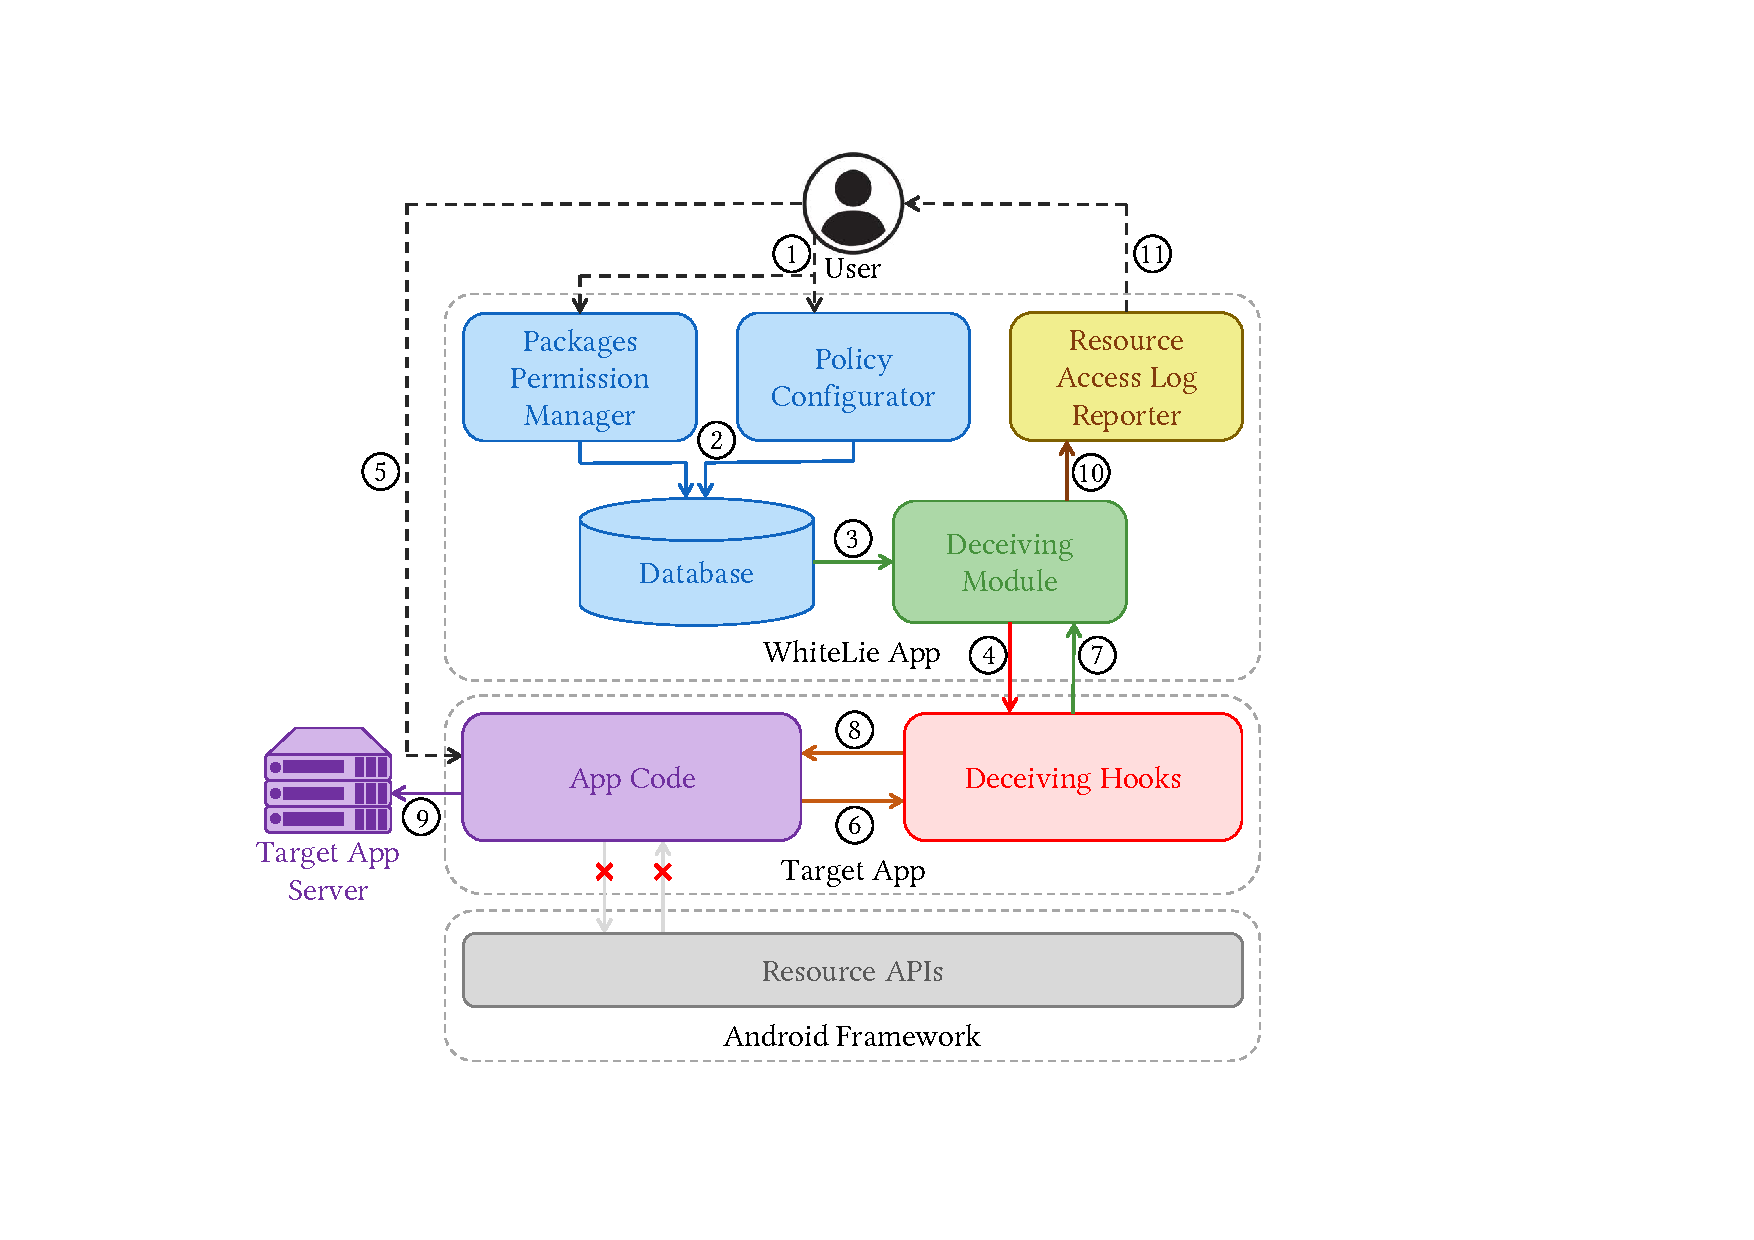
\includegraphics[width=0.75\linewidth]{Figures/Methodology/deceiver_working_architecture.pdf}
    \caption{\framework{} architecture.}
    \label{fig:method_frmwrkArch}
\end{figure}

\begin{figure}[t]
    \centering
    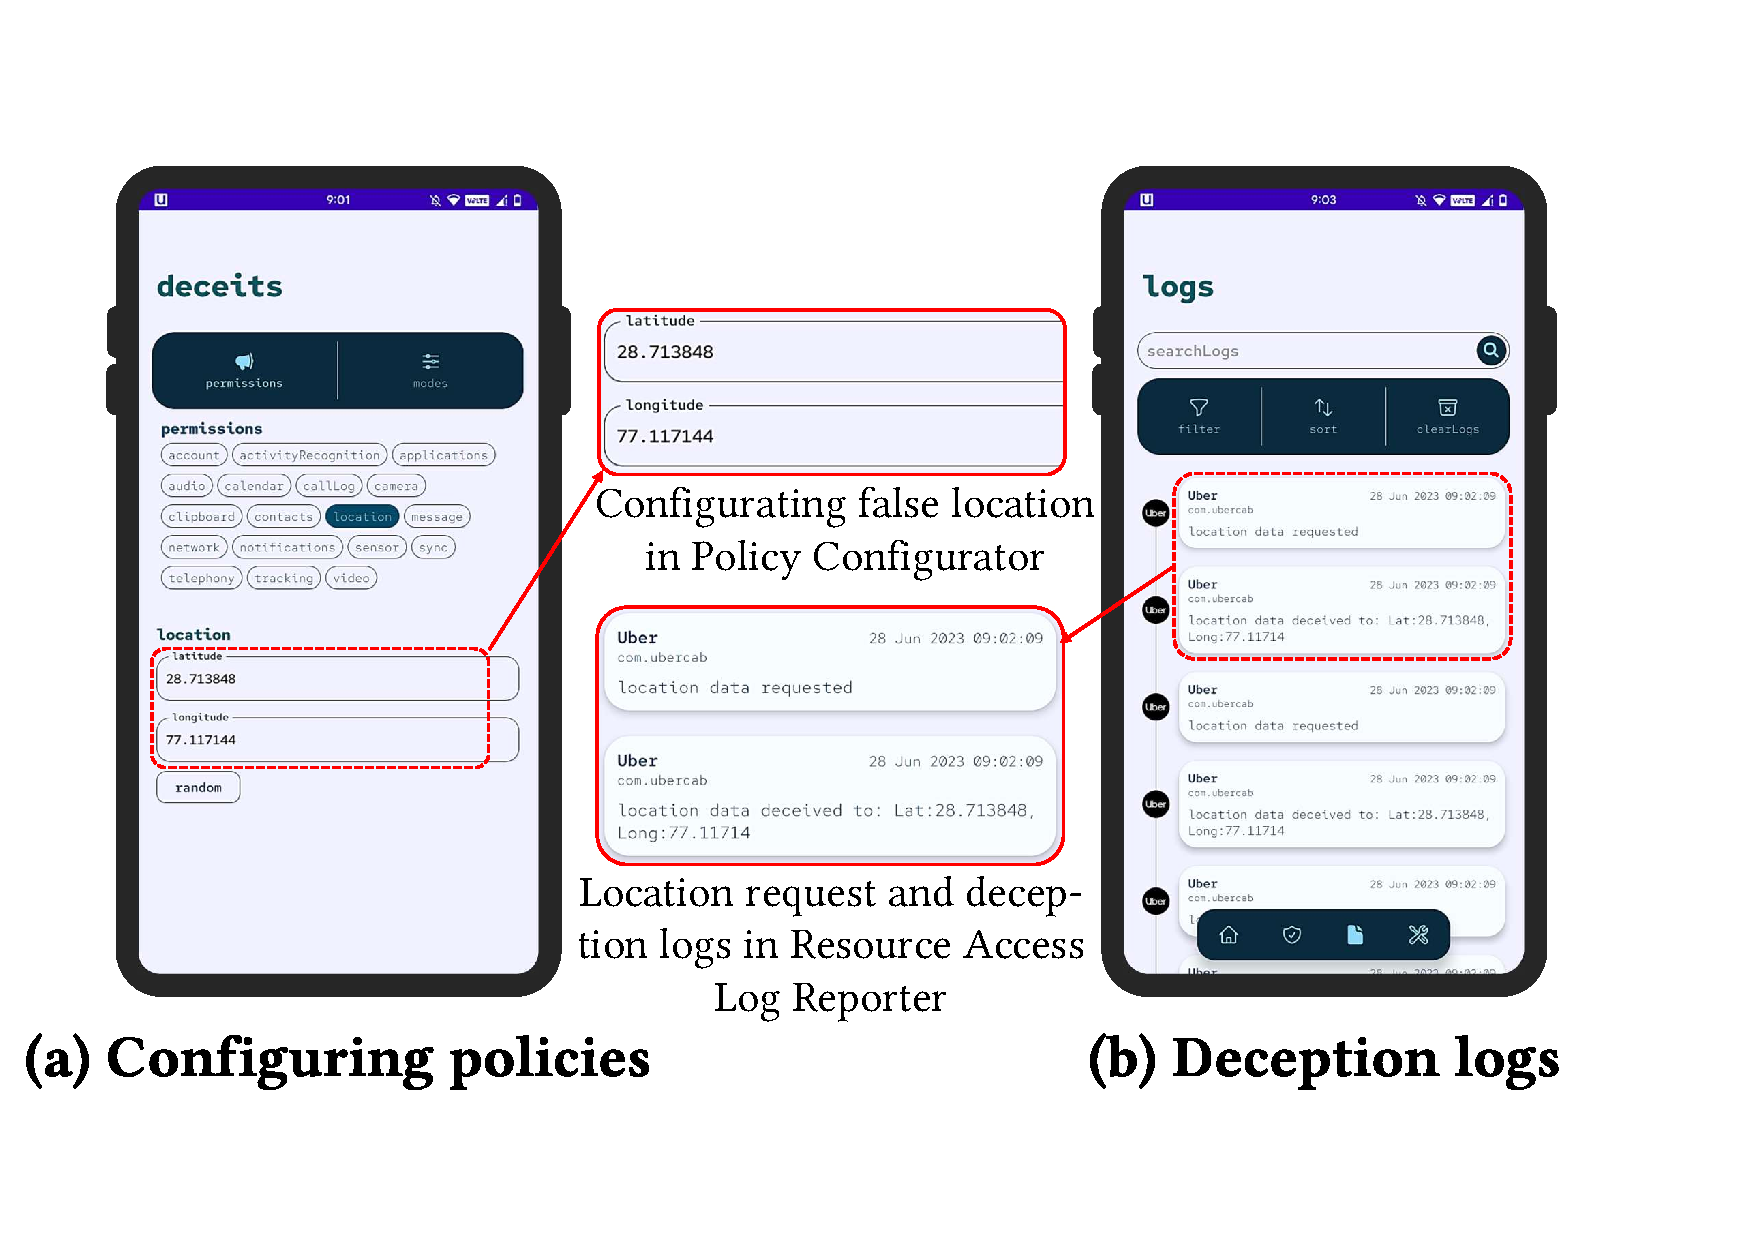
\includegraphics[width=0.75\linewidth]{Figures/Case Studies/whitelie_screenshots.pdf}
    \caption{Screenshots of \framework{} app UI while performing experiments to deceive location data for Uber.}
    \label{fig:frmwrk-ui}
\end{figure}

\circled{1}~To deceive the user data in the target apps, the user interacts with the \textit{Package-Permission Manager} to review the permissions requested and granted to the target package, listed by \framework{} using \textit{Query All Packages} permission (sole permission requested by \framework{}). The installed packages are fetched using \texttt{getInstalledApplication()} method configured for gathering metadata of installed applications. Then the user creates policies for the deceiving the user data associated with each permission. Figure~\ref{fig:frmwrk-ui}a presents the UI of \framework{}'s \textit{Policy Configurator} while defining the new deceit data for spoofing the location permission. Configuring policies enhances user's control over the spoofed data fed to apps by customizing the data, avoiding potential privacy compromises. 

\framework{} also streamlines the configuration of privacy policies by providing predefined 
%modes: Default, Random, and Intelligent. In Default mode, user data is deceived with pre-defined default values, while Random mode uses randomly generated data for obfuscation. The Intelligent mode employs pre-defined 
yet configurable set of meaningful real-world values and randomly selects to efficiently safeguard user data. For example, for Contacts permission, \framework{} has a set of 100 predefined real-world contacts, that are randomly fed to the target app when requested. \circled{2}~The \textit{Package-Permission Manager} and the \textit{Policy Configurator} stores the metadata and policies defined by the user in the database. 


% This module allows users to define policies for spoofing specific permissions within certain packages, which are stored in the \textit{App Policies} table and later utilised by the \textit{Spoofing Module} to determine which launched applications to affect and which permissions to deceive. 

 
% For example, when an app requests access to the contact list, \framework{} enables users to specify specific contacts to share instead of providing the entire list, reducing privacy risks.

% Configuring policies to ensure efficient privacy protection is a time-consuming task that demands technical knowledge of the Android Permission Framework and various Android resources. To streamline this process, the \framework{} incorporates predefined policies organised into distinct modes, namely: Default, Random, and Intelligent. Under Default mode, \framework{} deceives user data with default value, whereas in Random mode, user data is obfuscated with random information. And in Intelligent mode, \framework{} employs randomly selected meaningful real-world values to deceive user data.

When the target app is launched and its process is created, the \textit{XposedBridge} class is loaded along side in the process which makes the active Xposed modules, including the \framework{} to interact with the app.
\circled{3}~The \textit{Deceiving Module} of \framework{} fetches the policies defined by the user from the database and \circled{4}~accordingly installs the hooks in the target app.

\circled{5}~When the user interacts with the target app, \circled{6}~the app invokes the \textit{Deceiving Hooks} methods, instead of invoking the original sensitive Resource APIs. \circled{7}~These methods communicate with the \textit{Deceiving Module} via \texttt{ContentProvider} which references the stored policies to make informed decisions and sends over the policies back to the \textit{Deceiving Hooks}. \circled{8}~Consequently, the target app receives the deceived data rather than the original data from the hook method. \circled{9}~Hence, the target app sends deceived data over to its server, which ensures user data privacy. 

Additionally, the installed hooks also log the various actions performed by the hooked application with respect to user data access. \circled{10}~These logs are then relayed back to \framework{} when \textit{Deceiving Hooks} communicates with the \textit{Deceiving Module} during hooking. \circled{11}~These logs are shared with the user by the \textit{Resource Access Log Reporter} for manual investigation by the user. Figure \ref{fig:frmwrk-ui}b presents a screenshot of the \textit{Resource Access Log Reporter} logs recorded during the experiments.

% \subsubsection{Package-Permission Manager} 

% The user interacts with the Package-Permission Manager to review the permissions requested and granted to various packages. To gather information about installed packages and their permissions, \framework{} utilizes the \textit{Query All Packages} permission, which is the only permission requested by \framework{} app to accomplish its tasks. The installed packages are fetched using \texttt{getInstalledApplication()} method configured for gathering meta data of installed applications, storing the data in the \textit{Packages} table in the database. This module allows users to define policies for spoofing specific permissions within certain packages, which are stored in the \textit{App Policies} table and later utilised by the \textit{Spoofing Module} to determine which launched applications to affect and which permissions to deceive. Figure \ref{fig:frmwrk_ppm_ui} presents the UI of \framework{}'s \textit{Package-Permission Manager} while spoofing the location permission for \textit{Uber} app.

% \subsubsection{Policy Configurator} Once the package-permission policies are in place, users need to create policies for the deceived data associated with each permission. The \textit{Policy Configurator} facilitates this process, storing the policies in the \textit{Per App Permission Policies} table within the database. Figure \ref{fig:frmwrk_deciet_ui} presents the UI of \framework{}'s \textit{Policy Configurator} while defining the new deceit data for spoofing the location permission.

% Configuring policies to ensure efficient privacy protection is a time-consuming task that demands technical knowledge of the Android Permission Framework and various Android resources. To streamline this process, the \framework{} incorporates predefined policies organised into distinct modes, namely: Default, Random, and Intelligent. Under Default mode, \framework{} deceives user data with default value, whereas in Random mode, user data is obfuscated with random information. And in Intelligent mode, \framework{} employs randomly selected meaningful real-world values to deceive user data.

% \begin{figure}[t]
% \centering
% \begin{subfigure}{0.48\linewidth}
%     \centering
%     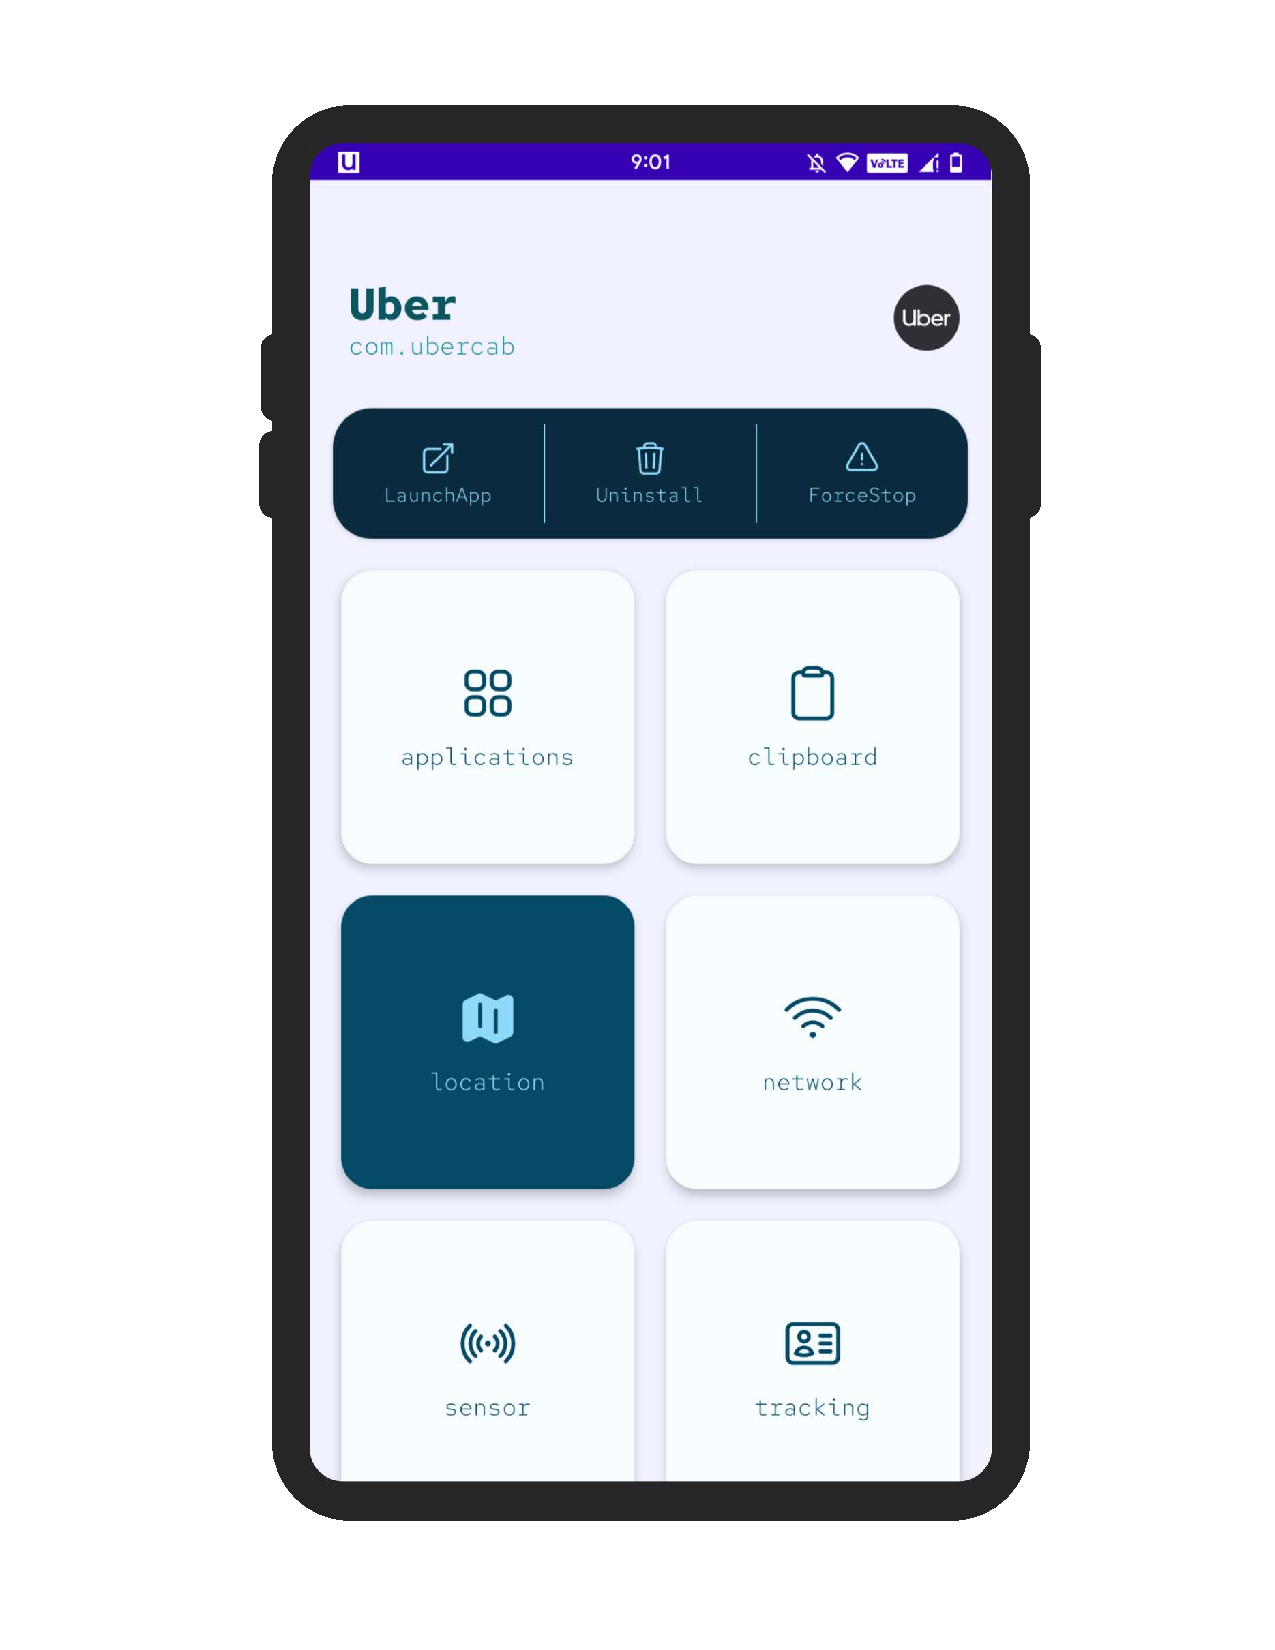
\includegraphics[width=0.8\linewidth]{figures/case_studies/uber_deceiving.pdf}
%     \caption{\framework{}'s \textit{Package-Permission Manager} to define spoofing policies}
%     \label{fig:frmwrk_ppm_ui}
% \end{subfigure}
% \begin{subfigure}{0.48\linewidth}
%     \centering
%     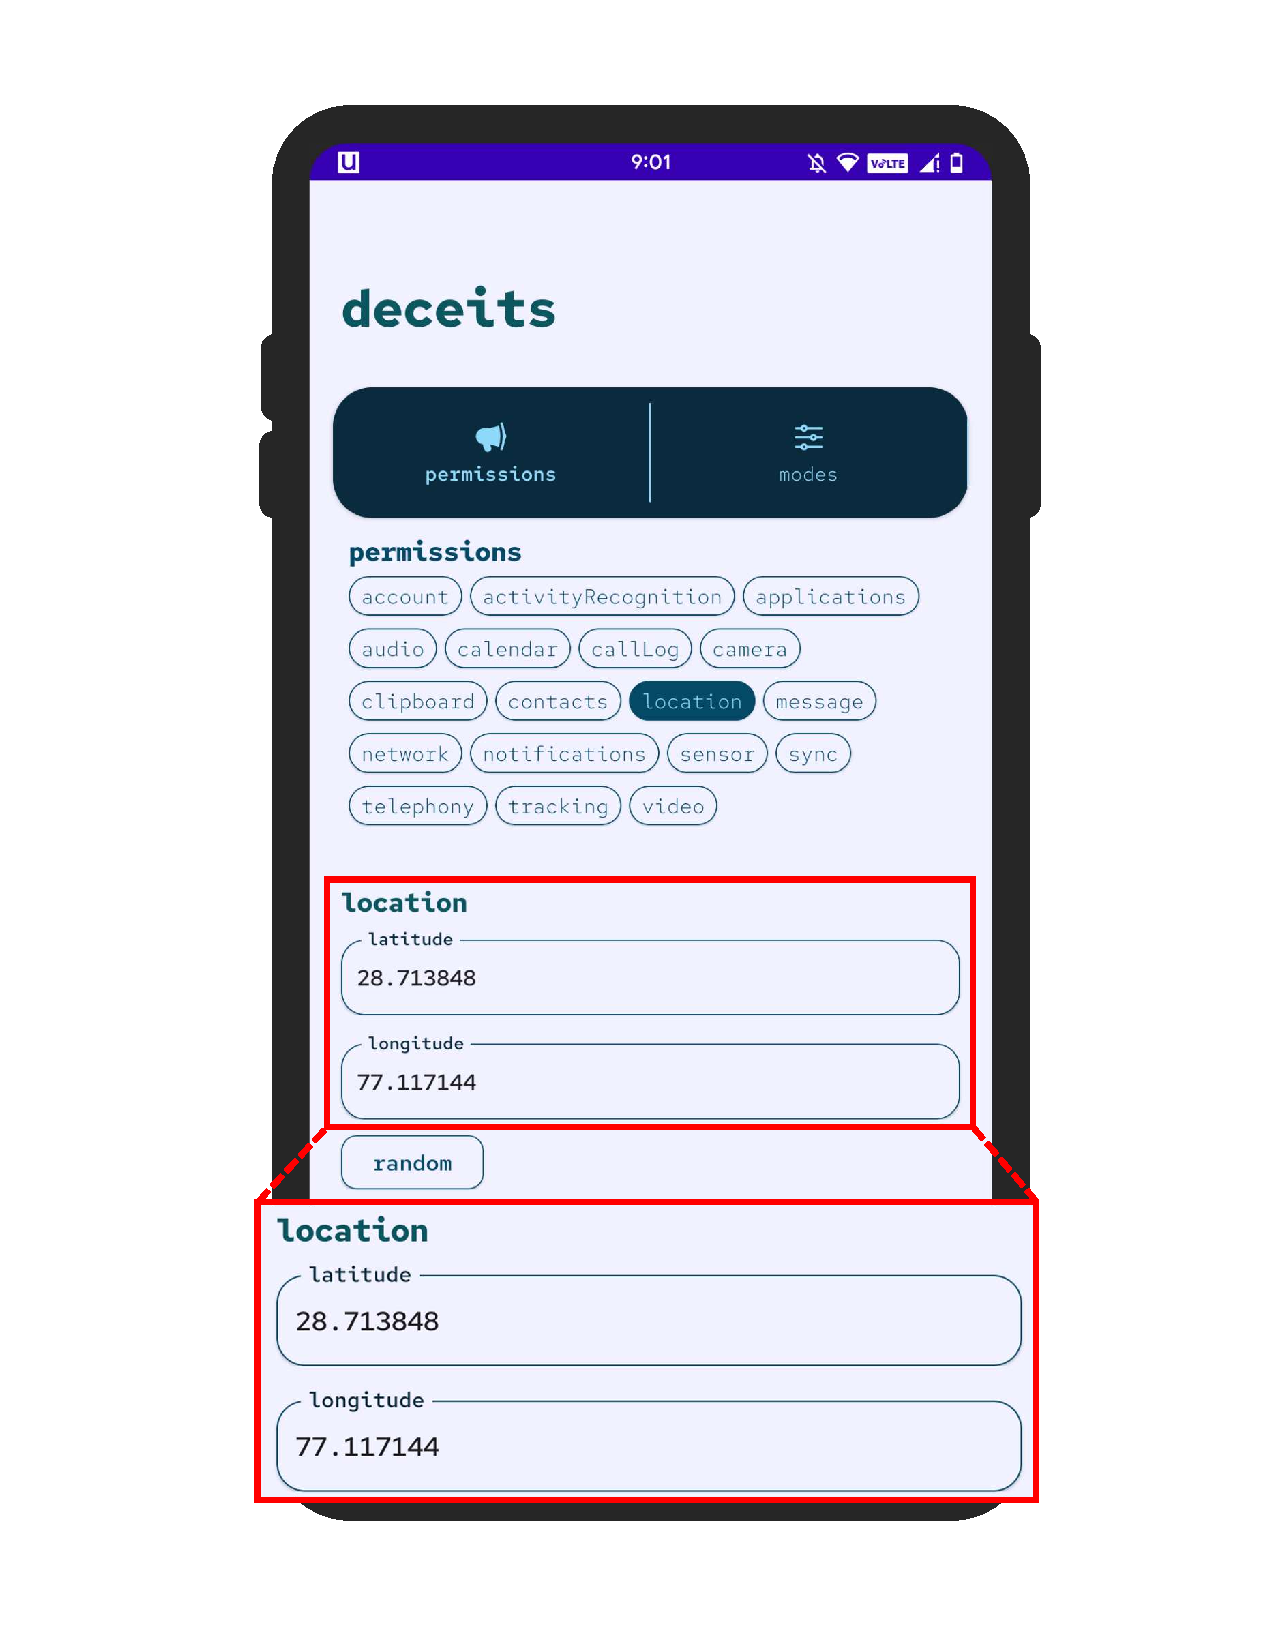
\includegraphics[width=0.8\linewidth]{figures/case_studies/uber_location_deceit.pdf}
%     \caption{\framework{}'s \textit{Policy Configurator} to define deceit data fed into target apps}
%     \label{fig:frmwrk_deciet_ui}
% \end{subfigure}
% \caption{Screenshots of \framework{} application UI while performing experiments to deceive location data for \textit{Uber}}
% \label{fig:frmwrk_ui}
% \end{figure}

% \subsubsection{Spoofing Module} The \textit{Spoofing Module} then references the policies during the hooking process to make informed decisions. When an app is launched and its process is created, the \textit{XposedBridge} class is loaded along side in the process which makes the active Xposed modules, including the \framework{} to interact with the app. This lets \framework{} to install the hooks based on policies in the target app. Subsequently, when the user interacts with the target app, and the app invokes the hooked methods, instead of invoking the original sensitive Resource APIs. Consequently, the target app receives deceived data rather than the original data.

% \subsubsection{Resource Access Log Reporter} Additionally, the installed hooks also logs the various actions performed by the hooked application with respect to user data access. These logs are then relayed back to the \framework{} via a \textit{Content Provider} and subsequently stored in the database in \textit{Resource Access Logs} table for manual investigation by the user through the \textit{Resource Access Log Reporter}. Figure \ref{fig:method_logReptr} presents a screenshot of the \textit{Resource Access Log Reporter} logs recorded during the experiments.

% \begin{figure}[t]
% \centering
% 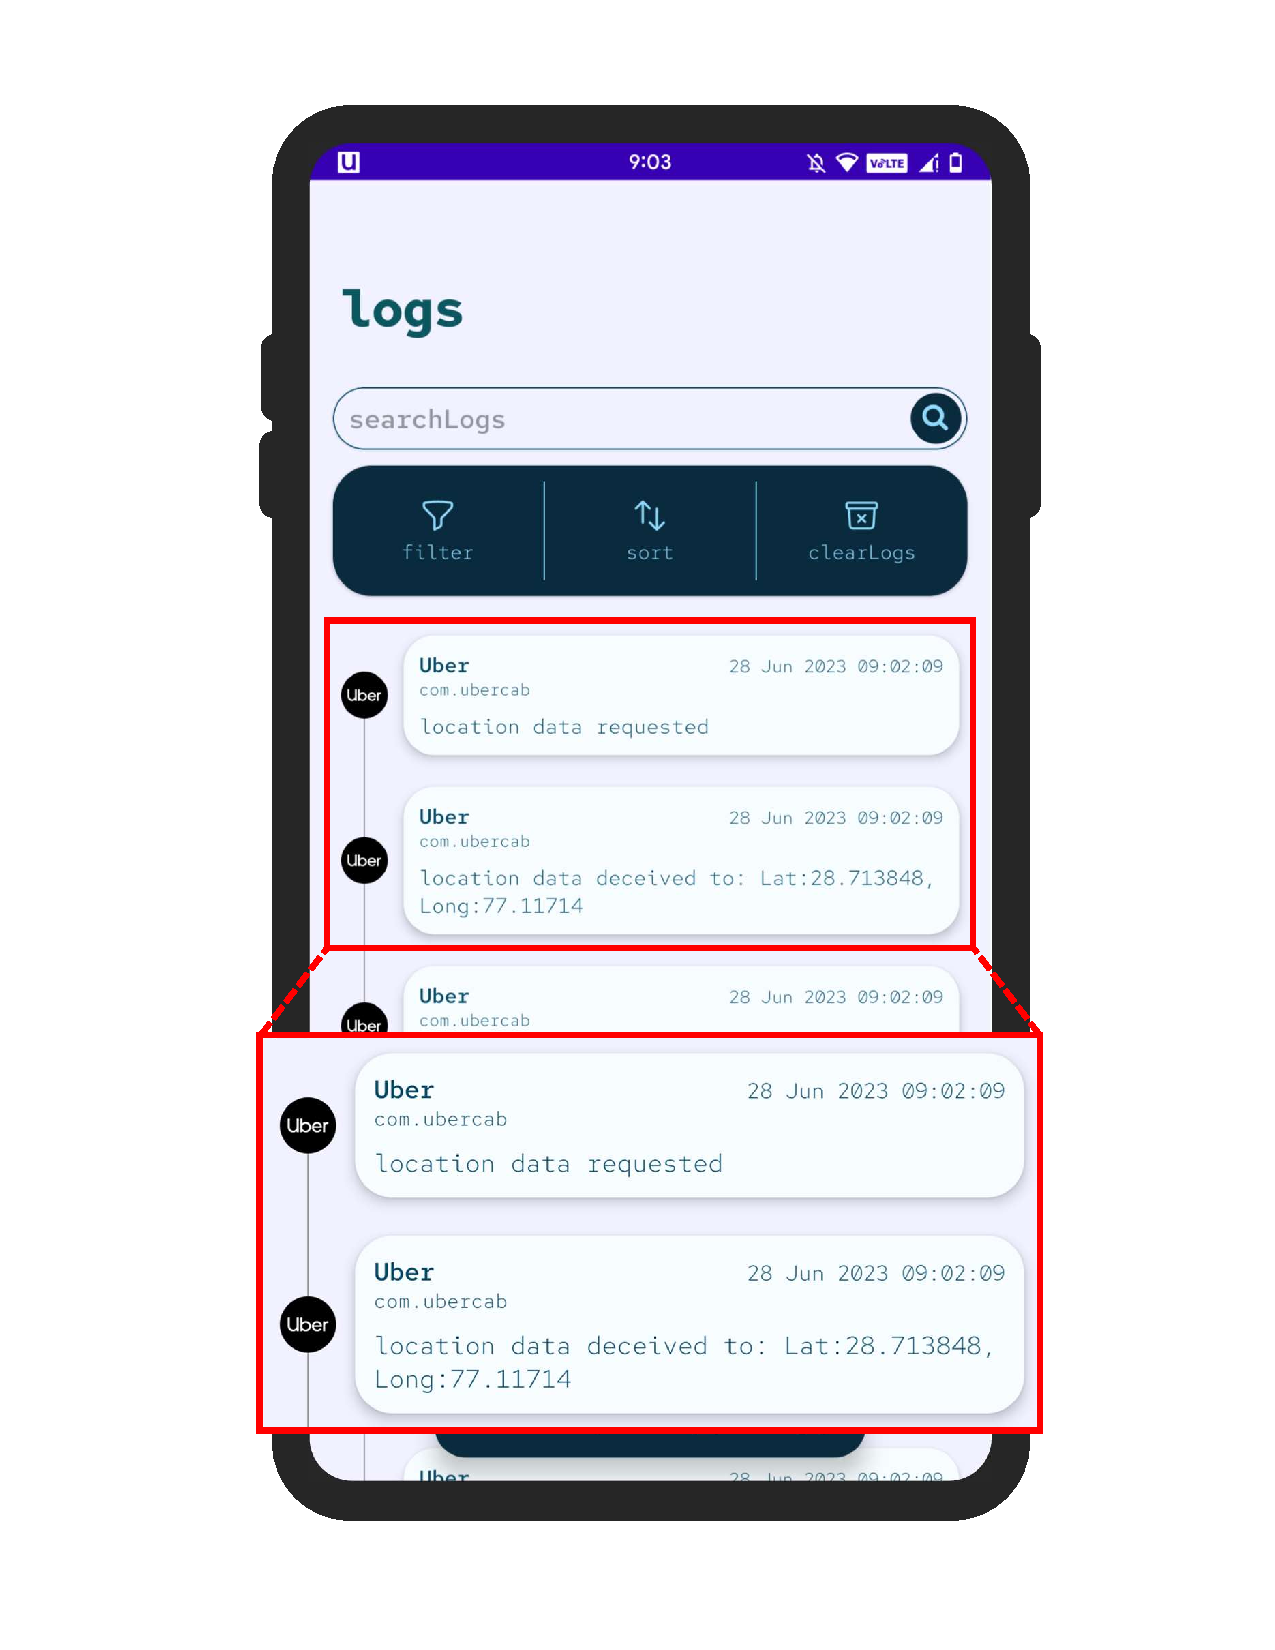
\includegraphics[width=0.384\linewidth]{figures/case_studies/uber_logs.pdf}
% \caption{Logs generated in the \framework{}'s \textit{Resource Access Log Reporter} for Location access and successful deception}
% \label{fig:method_logReptr}
% \end{figure}

% \subsection{User taking control over user data}
% \framework{} enhances user's control over the data supplied to various apps by offering an interface to define the data to be provided when apps request user data. Configuring policies enables users to understand the data shared with apps when user data is requested and define custom data to share, potentially privacy-compromising information. For instance, when an app requests the \textit{Read Contacts} permission to access the contact list, \framework{} allows users to define the contacts they want to share with the app instead of providing the complete contact list, which could pose privacy risks. The deceit data specified in the \textit{Policy Configurator} module is stored in the \textit{Content Provider} repository and can be queried by the hooks injected into targeted packages.